\documentclass[11pt,a4paper]{report}
\usepackage[spanish,es-nodecimaldot]{babel}	% Utilizar español
\usepackage[utf8]{inputenc}					% Caracteres UTF-8
\usepackage{graphicx}						% Imagenes
\usepackage[hidelinks]{hyperref}			% Poner enlaces sin marcarlos en rojo
\usepackage{fancyhdr}						% Modificar encabezados y pies de pagina
\usepackage{float}							% Insertar figuras
\usepackage[textwidth=390pt]{geometry}		% Anchura de la pagina
\usepackage[nottoc]{tocbibind}				% Referencias (no incluir num pagina indice en Indice)
\usepackage{enumitem}						% Permitir enumerate con distintos simbolos
\usepackage[T1]{fontenc}					% Usar textsc en sections
\usepackage{amsmath}						% Símbolos matemáticos
\usepackage{listings}

% Comando para poner el nombre de la asignatura
\newcommand{\asignatura}{Simulación de Sistemas}
\newcommand{\autor}{Vladislav Nikolov Vasilev}
\newcommand{\titulo}{PRÁCTICA 1}
\newcommand{\subtitulo}{Diferentes Modelos de Simulación}

% Configuracion de encabezados y pies de pagina
\pagestyle{fancy}
\lhead{\autor{}}
\rhead{\asignatura{}}
\lfoot{Grado en Ingeniería Informática}
\cfoot{}
\rfoot{\thepage}
\renewcommand{\headrulewidth}{0.4pt}		% Linea cabeza de pagina
\renewcommand{\footrulewidth}{0.4pt}		% Linea pie de pagina

\begin{document}
\pagenumbering{gobble}

% Pagina de titulo
\begin{titlepage}

\begin{minipage}{\textwidth}

\centering


\includegraphics[scale=0.5]{img/ugr.png}\\

\textsc{\Large \asignatura{}\\[0.2cm]}
\textsc{GRADO EN INGENIERÍA INFORMÁTICA}\\[1cm]

\noindent\rule[-1ex]{\textwidth}{1pt}\\[1.5ex]
\textsc{{\Huge \titulo\\[0.5ex]}}
\textsc{{\Large \subtitulo\\}}
\noindent\rule[-1ex]{\textwidth}{2pt}\\[3.5ex]

\end{minipage}

\vspace{0.5cm}

\begin{minipage}{\textwidth}

\centering

\textbf{Autor}\\ {\autor{}}\\[2.5ex]
\textbf{Rama}\\ {Computación y Sistemas Inteligentes}\\[2.5ex]
\vspace{0.3cm}


\includegraphics[scale=0.3]{img/etsiit.jpeg}

\vspace{0.7cm}
\textsc{Escuela Técnica Superior de Ingenierías Informática y de Telecomunicación}\\
\vspace{1cm}
\textsc{Curso 2018-2019}
\end{minipage}
\end{titlepage}

\pagenumbering{arabic}
\tableofcontents
\thispagestyle{empty}				% No usar estilo en la pagina de indice

\newpage

\setlength{\parskip}{1em}

\chapter{Mi primer modelo de Montecarlo}

\section{Pruebas iniciales con el modelo}

Inicialmente, se ha probado el modelo para ver cómo funcionaba. Se ha ejecutado el modelo una serie de
veces (10 para ser más precisos), y se han almacenado los resultados. La ejecución, suponiendo que
el programa ya estaba compilado, se ha hecho de la siguiente forma:

\begin{lstlisting}[language=bash]
$ for i in {1..10}; do \ 
bin/aparcamiento | tail -2 >> data/aparc-media.dat; \
done
\end{lstlisting}

Los resultados se muestran a continuación:

\begin{figure}[H]
\centering
\begin{tabular}{c|c}
\textbf{Mejor posición inicial ($c$)} & \textbf{Mejor distancia} \\ \hline
95                              & 6.525780                 \\
94                              & 6.472190                 \\
94                              & 6.513340                 \\
94                              & 6.531020                 \\
94                              & 6.498630                 \\
93                              & 6.512340                 \\
94                              & 6.469870                 \\
94                              & 6.487920                 \\
94                              & 6.486590                 \\
94                              & 6.478660                
\end{tabular}
\caption{Resultados de mejor posición inicial y mejor distancia para 10 ejecuciones.}
\end{figure}

Como se puede apreciar, parece que hay cierta semejanza entre los resultados obtenidos en cada
ejecución. Se puede ver que el valor de $c$ obtenido es muy similar en casi todos los casos, siendo
la moda $c = 94$, y la media un valor muy próximo a éste. Los valores de la mejor distancia también
son muy próximos entre sí, ya que todos ellos rondan, aproximadamente, las 6.5 plazas. Por tanto, el
modelo es capaz de producir unos resultados muy similares a pesar de que utiliza cierta ``aleatoriedad''.

Si estudiamos cómo evoluciona el valor de la distancia al destino a medida que cambia el valor de $c$, nos
encontramos con la siguiente gráfica:

\begin{figure}[H]
\centering
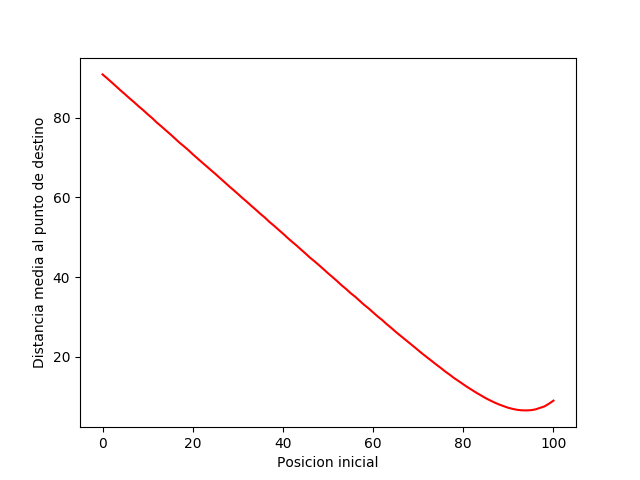
\includegraphics[scale=0.6]{img/c-dist.png}
\caption{Evolución del valor de la distancia al destino en función del valor de la posición inicial.}
\end{figure}

Como se puede ver, existe una tendencia a que, cuanto más cerca de la posición a la que se quiera llegar
se comienza a buscar sitio (es decir, cuanto más alto sea el valor de $c$), menor será la distancia hasta
el destino. Esto es completamente lógico, ya que al comenzar a buscar sitio a partir de una posición
muy lejana al destino, mayor será la distancia hasta éste en caso de que se encuentre una plaza libre. Teniendo
en cuenta que se escoge la primera plaza libre, ésta puede quedar muy lejos del destino, que es lo que se puede
apreciar en la gráfica.

El valor ideal de $c$, con las condiciones en las que estamos, parece ser $c = 94$. A partir de ahí, se puede ver
que existe un ligero incremento en la distancia al destino, posiblemente porque se aparque más lejos debido a que
no se encuentre una plaza libre en posiciones más cercanas al destino.

Por tanto, a vista de los resultados que hemos obtenido, podemos afirmar con bastante certeza que la plaza ideal
a partir de la que empezar sitio para aparcar es aproximadamente la 94.

\section{Experimentación con los parámetros}

\newpage

\begin{thebibliography}{5}

\bibitem{nombre-referencia}
Texto referencia
\\\url{https://url.referencia.com}

\end{thebibliography}

\end{document}

